%===============================================================================
% LaTeX sjabloon voor de bachelorproef toegepaste informatica aan HOGENT
% Meer info op https://github.com/HoGentTIN/bachproef-latex-sjabloon
%===============================================================================

\documentclass{bachproef-tin}

\usepackage{hogent-thesis-titlepage, float} % Titelpagina conform aan HOGENT huisstijl
\usepackage[shortlabels]{enumitem}
%%---------- Documenteigenschappen ---------------------------------------------
% De titel van het rapport/bachelorproef
\title{Application of professional webscraping in InsurTech}

% Je eigen naam
\author{Edouard Goddeeris}

% De naam van je promotor (lector van de opleiding)
\promotor{Benjamin Vertonghen}

% De naam van je co-promotor. Als je promotor ook je opdrachtgever is en je
% dus ook inhoudelijk begeleidt (en enkel dan!), mag je dit leeg laten.
\copromotor{Freek Verschelden}

% Indien je bachelorproef in opdracht van/in samenwerking met een bedrijf of
% externe organisatie geschreven is, geef je hier de naam. Zoniet laat je dit
% zoals het is.
\instelling{---}

% Academiejaar
\academiejaar{2021-2022}

% Examenperiode
%  - 1e semester = 1e examenperiode => 1
%  - 2e semester = 2e examenperiode => 2
%  - tweede zit  = 3e examenperiode => 3
\examenperiode{3}

%===============================================================================
% Inhoud document
%===============================================================================

\begin{document}

%---------- Taalselectie -------------------------------------------------------
% Als je je bachelorproef in het Engels schrijft, haal dan onderstaande regel
% uit commentaar. Let op: de tekst op de voorkaft blijft in het Nederlands, en
% dat is ook de bedoeling!

%\selectlanguage{english}

%---------- Titelblad ----------------------------------------------------------
\inserttitlepage

%---------- voorwoord --------------------------------------------
\usechapterimagefalse
%%=============================================================================
%% Voorwoord
%%=============================================================================

\chapter*{\IfLanguageName{dutch}{Woord vooraf}{Preface}}
\label{ch:voorwoord}

In het derde jaar Toegepaste Informatica wordt aan de Hogeschool Gent als eindwerk een scriptie verwacht, relevant aan de opleiding. Als projecten buiten school ben ik al altijd gefascineerd geweest door automatisatie. Dit gaat dan over autoclickers op computerspellen of het opsommen van data zonder te moeten manueel kopiëren en plakken. In het kort, herhaaldelijke taken uitsluiten door efficiënter een computer te gebruiken. In mijn vrije tijd heb ik vaak al kleine projecten uitgeschreven om te achterhalen hoe ik telkens kleine zaken kan automatiseren. Ook als specialisatie Data Engineer en AI leek het zeer gepast een aansluiten onderzoek hierover te doen. Tijdens het tweede semester werd van mij verwacht dat ik stage zou lopen bij een informatica bedrijf. Ik ging op zoek in Gent naar een bedrijf die aan mijn interesses voldeed. Zo kwam ik bij WeGroup terecht, een startup InsurTech bedrijf die een verzekeringstool aanbiedt voor verzekeringsmakelaars. Tijdens mijn eerste week stage had ik al snel het idee om onderzoek te doen die een combinatie is van de branche waarin mijn stagebedrijf zit en mijn passie voor data en automatisatie. Zo kwam ik bij webscraping en de toepassingen ervan binnen de InsurTech.

Deze bachelorproef had ik niet alleen kunnen uitwerken. Daarom bedank ik graag mijn stagebegeleider bij WeGroup Freek Verschelden die me duidelijkheid bracht over InsurTech en de tools die binnen het bedrijf gebruikt worden of al geïmplementeerd waren.
Ook bedank ik graag mijn co-promotor Benjamin Vertonghen die me concreet feedback en inspiratie gaf bij waar ik precies met mijn onderzoek naartoe wou.



%---------- Inhoudstafel -------------------------------------------------------
\pagestyle{empty} % Geen hoofding
\tableofcontents  % Voeg de inhoudstafel toe
\cleardoublepage  % Zorg dat volgende hoofstuk op een oneven pagina begint
\pagestyle{fancy} % Zet hoofding opnieuw aan

%---------- Lijst figuren, afkortingen, ... ------------------------------------

% Indien gewenst kan je hier een lijst van figuren/tabellen opgeven. Geef in
% dat geval je figuren/tabellen altijd een korte beschrijving:
%
%  \caption[korte beschrijving]{uitgebreide beschrijving}
%
% De korte beschrijving wordt gebruikt voor deze lijst, de uitgebreide staat bij
% de figuur of tabel zelf.

\listoffigures
\listoftables
\lstlistoflistings

% Als je een lijst van afkortingen of termen wil toevoegen, dan hoort die
% hier thuis. Gebruik bijvoorbeeld de ``glossaries'' package.
% https://www.overleaf.com/learn/latex/Glossaries

%---------- Kern ---------------------------------------------------------------

% De eerste hoofdstukken van een bachelorproef zijn meestal een inleiding op
% het onderwerp, literatuurstudie en verantwoording methodologie.
% Aarzel niet om een meer beschrijvende titel aan deze hoofstukken te geven of
% om bijvoorbeeld de inleiding en/of stand van zaken over meerdere hoofdstukken
% te verspreiden!

%%=============================================================================
%% Inleiding
%%=============================================================================

\chapter{\IfLanguageName{dutch}{Inleiding}{Introduction}}
\label{ch:inleiding}

De Insurance Technology is een vooruitstrevende technologie die in de verzekeringswereld gebruikt wordt. Verzekeringsmaatschappijen willen voortdurend op kosten en tijd besparen, dit is net waar de InsurTech zich op focust. Eerst en vooral werd onderzocht hoe een standaard verzekeringsproces precies verloopt en welke documenten en voornamelijk welke informatie hiervoor ingevuld moet worden. Vervolgens werd gezocht naar welke stadia in dit proces geautomatiseerd of versneld konden worden. Dan zal voor deze onderdelen een automatisatie gezocht worden die men verwerft via data die men via webscraping of het gebruik van Application Programming Interfaces (API’s) op externe webpagina’s verkrijgt. Het onderzoek zou een oplossing moeten bieden voor het lange “invulproces” die de klant en de makelaar moeten doorlopen om een verzekeringscontract op punt te zetten. De verzekeringswereld krijgt de voorbije decennia te maken met een ware opmars in technologiegebruik. Het opstellen en invullen van verzekeringscontracten vereist contact met de klant, hier kan innovatieve technologie aan de pas komen . Het onderzoek zou een steentje moeten bijdragen aan de mogelijke methodes waarin dit proces kan versneld worden waarbij tools zoals Selenium en Puppeteer gebruikt worden. Bij het gebruik API’s maakt dit onderzoek gebruik van de requests library in Python indien webscraping niet nodig of mogelijk is. Verder zal voor het onderzoeken van externe Application Programming Interfaces (API’s) de Google Developer Tools een hulp bieden in het uitwerken van de toepassingen. Als eindresultaat zal een minimalistische simulatie aantonen dat de toepassing wel degelijk innovatief is.

\section{\IfLanguageName{dutch}{Probleemstelling}{Problem Statement}}
\label{sec:probleemstelling}

De verzekeringswereld heeft de afgelopen decennia technologische vooruitgang geboekt.
In deze wereld willen de verzekeringsmakelaars voortdurend op geld en tijd sparen. Het liefst herinvesteren ze deze dan terug in hun klanten om deze tevreden te houden. De nood aan nieuwe technologieën die makelaars deze herinvestering kunnen aanbieden is erg van belang. Wegens dat deze Insurance technologie nog vrij nieuw is, liggen er nog vele kansen voor het grijpen voor software ontwikkelaars om een tool of toepassing te ontwikkelen die het voor deze makelaars, alsook uiteindelijk de klant, gemakkelijker zou maken een verzekeringscontract af te sluiten. Vandaar gaat dit onderzoek uit op één of meerdere toepassingen die de efficiëntie in de verzekeringswereld technologisch kan bevorderen. Dit kan gaan van het vereenvoudigen van formulieren tot het automatiseren van manuele herhaaldelijke taken door middel van webscraping.

\section{\IfLanguageName{dutch}{Onderzoeksvraag}{Research question}}
\label{sec:onderzoeksvraag}

Het uiteindelijke doel van dit onderzoek bestaat eruit om een inzicht te geven over welke toepassingen mogelijk zijn in de Insurtech via webscraping met daarbovenop nog een prototype van een onbestaande toepassing. Om een zo duidelijk mogelijk antwoord te bieden op de onderzoeksdoelstelling van dit onderzoek, werden volgende onderzoekvragen opgesteld:
\begin{itemize}
	\item Welke toepassingen bestaan reeds in de InsurTech?
	\item Welke nieuwe toepassingen zijn er mogelijk via webscraping?
	\item Wat betreft de tijdswinst van deze nieuwe toepassing?
\end{itemize}

\section{\IfLanguageName{dutch}{Onderzoeksdoelstelling}{Research objective}}
\label{sec:onderzoeksdoelstelling}

Het beoogde eindresultaat van dit onderzoek omvat minstens één nuttige technologie waarbij webscraping werd gebruikt die het werk voor een verzekeringsmakelaar bevordert. De efficiëntie is merkbaar doordat een manueel proces geautomatiseerd of geoptimaliseerd is dankzij de gebruikte toepassing. Deze toepassing is door middel van een prototype onderzocht, geschreven in de programmeertaal Python.

\section{\IfLanguageName{dutch}{Opzet van deze bachelorproef}{Structure of this bachelor thesis}}
\label{sec:opzet-bachelorproef}

% Het is gebruikelijk aan het einde van de inleiding een overzicht te
% geven van de opbouw van de rest van de tekst. Deze sectie bevat al een aanzet
% die je kan aanvullen/aanpassen in functie van je eigen tekst.

De rest van deze bachelorproef is als volgt opgebouwd:

In Hoofdstuk~\ref{ch:stand-van-zaken} wordt een overzicht gegeven van de stand van zaken binnen het onderzoeksdomein, op basis van een literatuurstudie. Hierbij worden de bestaande toepassingen van de Insurtech besproken alsook alles omtrent webscraping om het vervolg van het onderzoek te begrijpen.

In Hoofdstuk~\ref{ch:methodologie} wordt het onderzoek voorbereid en de toepassingen besproken om een antwoord te kunnen formuleren op een deel van de onderzoeksvragen.

In Hoofdstuk~\ref{ch:voorbereiding-onderzoek} wordt kort de relevantie van data besproken en de toepassingen van InsurTech.

In Hoofdstuk~\ref{ch:prototype} wordt een prototype van een toepassing binnen de InsurTech ontwikkeld waarbij webscraping en mogelijke struikelblokken worden toegelicht. Hierbij wordt in detail de werkwijze alsook de code uitgelegd die voor resultaten zorgt omtrent de optimalisatie van een verzekeringsproces.

In Hoofdstuk~\ref{ch:conclusie}, tenslotte, wordt de conclusie gegeven en een antwoord geformuleerd op de onderzoeksvragen. Daarbij wordt ook een aanzet gegeven voor toekomstig onderzoek binnen dit domein.
\chapter{\IfLanguageName{dutch}{Stand van zaken}{State of the art}}
\label{ch:stand-van-zaken}

% Tip: Begin elk hoofdstuk met een paragraaf inleiding die beschrijft hoe
% dit hoofdstuk past binnen het geheel van de bachelorproef. Geef in het
% bijzonder aan wat de link is met het vorige en volgende hoofdstuk.

% Pas na deze inleidende paragraaf komt de eerste sectiehoofding.

In dit hoofdstuk worden de verschillende termen die aan de InsurTech en Webscraping gebonden zijn uitvoerig besproken.

\section{InsurTech}

Allereerst wordt de term InsurTech verklaard.
InsurTech is een porte-manteauwoord van insurance en technology.
Concreet is dit het introduceren of gebruik maken van innovatieve technologie in de verzekeringswereld.
Deze innovatieve technologiën worden ontwikkeld door middel van het gebruik van apps, Big Data, machine learning, draagbare producten zoals smartwatches en andere transformatieve technologiën die processen betreffende de verzekeringswereld kunnen automatiseren of bevorderen. Deze bevorderingen kunnen gaan van 
De InsurTech is in principe een specialisatie van FinTech, ofwel Financial Technology.
Terwijl FinTech zich op alle financiële technologieën focust, beperkt de InsurTech zich tot die van de verzekeringswereld.
Een duidelijk verschil is dat de FinTech onder meer ook nog over technologie in banken gaat.

InsurTech is nog vrij nieuw, zo worden er regelmatig nieuwe toepassingen ontwikkeld die de efficiëntie van een verzekeringsbedrijf bevordert. Zo wijst een artikel van \textcite{Institute2020} erop dat de term is opgekomen rond 2010, toen de hoofdimplementatie eerder prijsvergelijkingen tussen verschillende verzekeringsmaatschappijen was. Tegenwoordig reiken de toepassingen van InsurTech veel verder dan alleen prijsvergelijkingen, zoals verzekeringsadvies bieden op basis van verzamelde data. Een ander artikel uit 2021 of \textcite{InsuranceCommissioners2021} toont aan dat InsurTech startups de voorbije decennia een geschatte 16,5 miljard dollar aan investeringen hebben verzameld en dat dit bedrag in de toekomst alleen maar zal groeien. Een literatuurstudie van \textcite{inproceedings} concludeert dat de verzekeringsmaatschappijen vooral kosten, in tijd en geld, verliezen door het analyseren van de risico’s die een klant loopt om zo de juiste verzekeringen aan te raden. Door InsurTech toepassingen is het beheren van verzekeringen en de klantencommunicatie niet alleen vergemakkelijkt, maar ook verbeterd. Wat webscraping en datamining betreft bestaat er reeds een grote variëteit aan technologie en tools. Er zal zowel voor een toepassing voor webscraping, als API gebruik gezocht worden bij het vinden van een toepassing die de klantenervaring kan bevorderen.

\subsection{De werking van verzekeringen}
Een verzekering wordt door \textcite{Trowbridge1975} omschreven als een risico-overdracht waarbij
een klant het risico overdraagt aan een verzekeringsmaatschappij in ruil voor een overeengekomen bedrag. 
Het doel van de klant in dat geval is de negatieve financiële gevolgen te beperken van een onzekere toekomstige gebeurtenis.
\graphicspath{ {./img/} }
\begin{figure}[H]
	\centering
	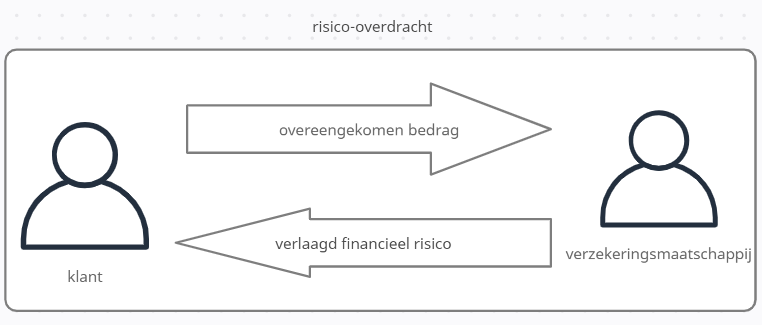
\includegraphics{creately_basic_verzekering}
	\caption{Verzekering visualisatie volgens \textcite{Trowbridge1975}}
\end{figure}
Een verzekering krijgt volgens \textcite{cortis2019insurtech} verder ook de taak en verantwoordelijkheid een inschatting te maken over welk bedrag opgesteld moet worden. Dit is afhankelijk van de grootte van het risico die de verzekeringsmaatschappij met zich meedraagt. Wanneer een klant zijn vergoeding opeist, wordt bij de verzekering een claim management proces opgesteld. Dit is opnieuw één van de processen waar tijd- en kost-efficiëntie een rol speelt.



\section{Webscraping}

Allereerst gaan we terug in de tijd, naar het ontstaan van webscraping. Webscraping dateert al van het begin van het World Wide Web, ontstaan in 1989, toen het internet voor het eerst werd geïntroduceerd. Nog geen 4 jaar later, in 1993, werd al voor het eerst de term “webscraping” gebruikt. Het jaar waarin een groep MIT (Massachusetts Institution of Technology) studenten als schoolproject de omvang van het internet probeerden in te schatten. Hun allereerste webscraper, de World Wide Web Crawler, werd de basis van vele andere webscrapers die nog in de toekomst zouden volgen. In datzelfde jaar werd alsook de allereerste zoekmachine op het internet uitgevonden door Jonathan Fletcher, de “vader van de zoekmachine”. Deze student aan de University of Sterling te Schotland ontwierp onbewust de voorloper van Google genaamd Jumpstation. \autocite{farholt2021less} Mettertijd is het gebruik van webscraping en de gebruikte toepassingen drastisch gewijzigd. Zo worden tegenwoordig webscrapers gebruikt om interactie van een gebruiker te simuleren om webpagina’s uit te testen vanuit het standpunt van de eindgebruiker.
Webscraping is reeds heel wat geëvolueerd, zo moet de technologie zich vaak aanpassen aan hoe webpagina’s eigenlijk opgebouwd zijn.
Webscraping is het extraheren en indexeren van data in webpagina’s en deze vervolgens opslaan in een tekstbestand of databank. Webpagina’s bestaan uit tekst die in verschillende formaten beschikbaar is: als gewone tekst, in tabellen, ... De simpelste vorm van webscraping het kopiëren en plakken van tekst. Het is de taak van een webscraper deze data automatisch uit te lezen en te indexeren. Het crawlen of scrapingsproces op het internet bestaat er allereerst uit alle gewenste data uit te lezen om deze vervolgens in een gepast leesbaar formaat te structureren.\autocite{zhao2017web} Hoofdzakelijk wordt dit gebruikt om repetitieve taken te versnellen, zoals iedere subtitel van een pagina kopiëren en plakken. Het uitlezen kan op verschillende manieren gebeuren, afhankelijk van de desbetreffende webpagina. Echter is het niet hoofdzakelijk nodig altijd webscraping toe te passen. Soms beschikt de webpagina of service over een API, een acroniem voor Application Programming Interface. Dit is een set van functies en procedures gebruikt die één of meerdere taken vervuld met als doel door software gebruikt te worden. Dit maakt het voor programmeurs makkelijker en efficiënter om net de data die men nodig heeft uit de pagina te halen zonder overbodige data ook nog in te laden. Performantiegewijs heeft het gebruik van API’s op webpagina’s of services duidelijk de voorkeur. \autocite{10.2307/251584}
Abstract kan het gebruik van webscraping vanalles inhouden. Kleinschalig kan dit gaan over het monitoren van real-time data met behulp van polling, wat een detectiesysteem kan inhouden die aanpassingen op websites detecteert. Tot grootschalig het voortdurend uitlezen van website data om een zoekmachine mee te bouwen. Zo kan Google of Bing aanzien worden als één grote webscraper, gebruikt om het internet uit te mappen. \autocite{snyder2003web}

\begin{figure}[bh]
	\centering
	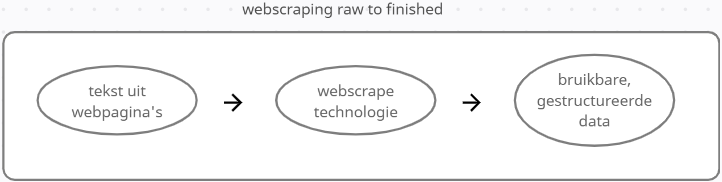
\includegraphics{webscraping_cycle}
	\caption{webscraping structuur}
\end{figure}

\subsection{Populaire Webscrapers}

% TODO leg uit waarom er gekozen werd voor enkel Selenium en puppeteer uit te leggen dmv populariteit
Een recent onderzoek duidt aan dat Selenium en Puppeteer tussen de populaire webscrapers zitten. (Saurkar e.a., 2018)


\subsection{Puppeteer}

% TODO vul aan wat Puppeteer is
Puppeteer

\subsection{Selenium}

Selenium is een web-UI testing library, wat wil zeggen dat de library geschikt is voor testdoeleinden. Selenium is echter niet beperkt tot deze doeleinden. Het is een set van verschillende software tools die elk een verschillende aanpak hebben om geautomatiseerde testen te ondersteunen. Het geautomatiseerd testen is de techniek van het automatiseren van de uitvoerings van testgevallen met behulp van gespecialiseerde software. Het feit dat deze library ondersteund wordt in verschillende webbrowsers maakt de library zeer toegankelijk.

\begin{figure}[bh]
	\centering
	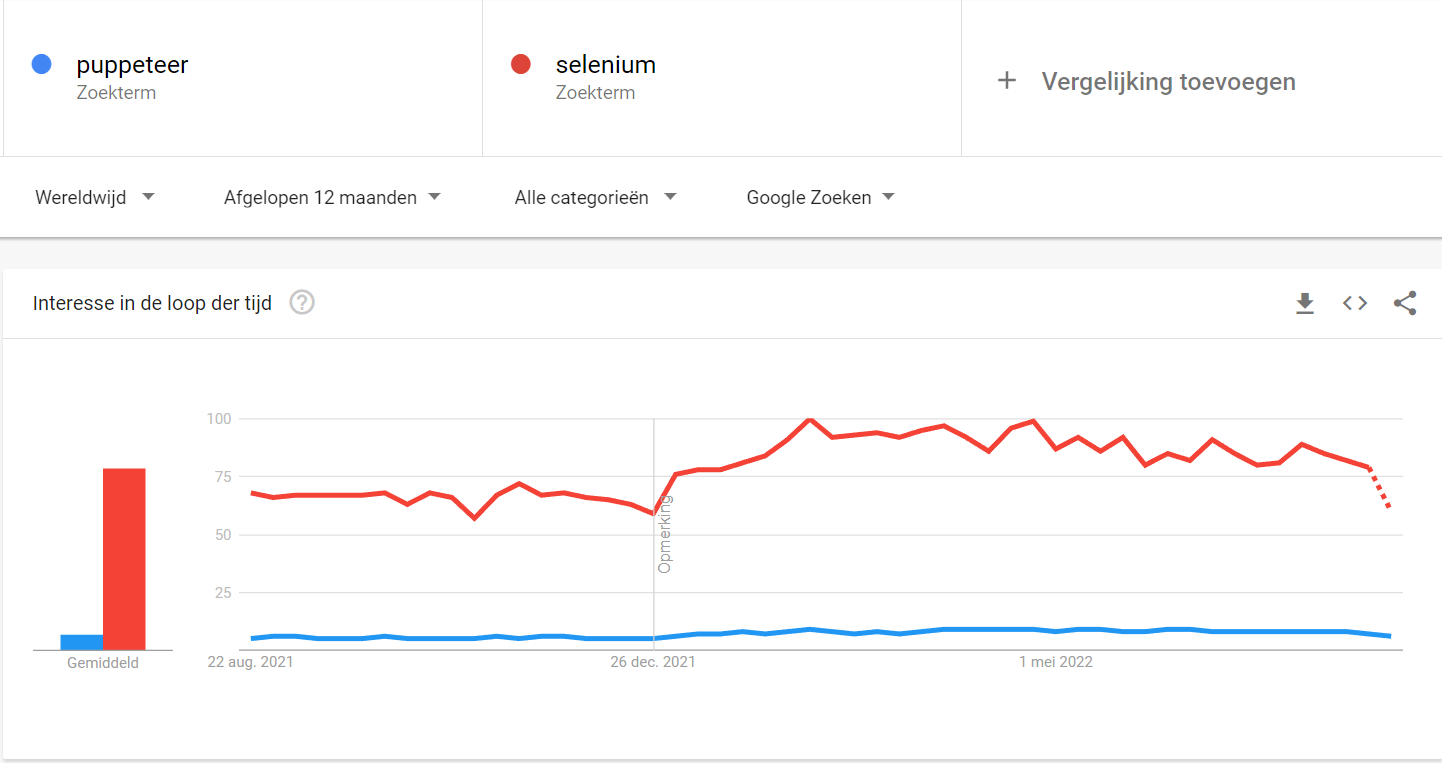
\includegraphics[width=\paperwidth, height=\textheight, keepaspectratio]{selenium_puppeteer_google_trends}
	\caption{Vergelijking Selenium vs Puppeteer op \href{https://trends.google.com/trends}{Google Trends}}
\end{figure}

\section{Databanken}

Er worden steeds meer gegevens verzameld en gebruikt, mede door middel van hierboven beschreven webscrapers. Als gevolg daarvan zijn databanken belangrijker dan ooit.
Om  data op te slaan is nood aan gestructureerde opslag, zodat de inhoud ervan makkelijk toegankelijk en beheerbaar is. 

Opslag van data in een soort databanken bestaat al enkele millenia. De Egyptenaren zouden de voorvaders kunnen genoemd worden in het opslaan van data. Ze hielden informatie bij door in stenen te kerven of op dierenhuiden te schrijven. Flash forward naar de 21e eeuw en er zijn al heel wat nieuwe modernere methoden om data op te slaan, voornamelijk op computers met gebruik van een databank.
Een databank is een collectie van deze data, waarin data records of bestanden door een databank manager worden beheerd. \autocite{obenshain_2004} Databanken worden gebruikt om gegevens efficiënt op te slaan en op verzoek alle data of een delen ervan terug te bezorgen. Databank tools bevatten gebruikelijk een zoekfunctie waarbij vragen zoals "Wie heeft het voorbije jaar een verzekeringscontract afgesloten?" kunnen beantwoord worden. Deze databanken worden voornamelijk gebruikt binnen grote mainframe systemen, alsook kleinere systemen of persoonlijke computers. Het is nutteloos als ze in een database zitten en niets doen. Er wordt gebruik gemaakt van software om er iets van te maken. Software formatteert deze opgeslagen data en structureert ze op een manier die zinvol is en ons in staat stelt weloverwogen beslissingen te nemen.

% TODO: voeg databank figure toe met fields en records voorbeeld

\section{Datamining}

Datamining is een multidisciplinair gebied dat statistiek, databanktechnologie, patroonherkenning, machine learning, gegevensvisualisatie en expertise in systemen omvat.
Wanneer een onderzoek werkt met grote datasets, is het manueel nagaan van verbanden ingewikkeld en heeft de data dus als vereiste automatisch gecontroleerd te worden.
Datamining bestaat uit het onderzoeken van bestaande data uit grote bestaande databanken, met als doel nieuwe data te genereren. Datamining is eerder waardevol voor gecompliceerdere zoektermen, zoals "Welk verband kan gevonden worden tussen de verzekeringscontracten die afgesloten werden het voorbije jaar?".
Op zichzelf is datamining een proces waar, in een grote set data, onderzoek wordt gedaan naar nuttige, relevante data. Het vinden van patronen, algoritmes en afwijkingen in deze grote set data moeten hierbij helpen. Het doel van de datamining techniek is om net ongekende patronen te vinden in de set data om deze vervolgens met elkaar te kunnen linken en structureren. Dit kan dan een antwoord bieden op business gerelateerde vragen die te tijd consumerend zijn om zelf op te lossen. \autocite{osman2019data} In detail kan dit logisch proces is onderverdeeld in 2 delen: het wetenschappelijke en het commerciële. Voornamelijk zijn toepassingen die het dataminen bevorderen in de InsurTech voornamelijk gefocust op het commerciële. \autocite{hand2007principles}

\subsection{Datamining proces}

Om datamining om te zetten in praktijk, namelijk van het extraheren van data tot het visualiseren ervan, worden een aantal stappen ondernomen.


\section{Webscraping vs Datamining}

Nu voorgaande termen onderling zijn besproken, wordt het verschil of de samenhang van beiden besproken. In het kort werd webscraping eerder omschreven als een data ophalen. Terwijl webscraping eerder het ophalen van data is en formatteren doet het geen analyse of dataprocessing. Het is net de datamining die de opgehaalde data zal verrijken en hieruit conclusies, verbanden en verschillen uit zal halen. In feite kan web scraping dus gebruikt worden om datasets te creeëren waarop datamining wordt toegepast. Deze beiden vullen elkaar dus aan.


\section{Tools}

Bij webscraping is het belangrijk om de juiste tool te vinden die voldoet aan jouw benodigdheden.
Zo is het bij dit onderzoek de bedoeling enkel webscrapers te gebruiken die draaien op de programmeertaal Python, dus is \href{https://nutch.apache.org}{Apache Nutch} bijvoorbeeld al niet van toepassing. Zo zijn er nog vele andere webscraping tools die \textcite{Sirisuriya2015} aanhaalt in haar studie.
Bij een recent onderzoek naar de meestgebruikte tools in Python kwamen Selenium en Puppeteer als één van de populairste uit de bus. \autocite{Saurkar2018}
Vandaar zal ook bij dit onderzoek deze tools gebruikt worden. Deze maken gebruik van webautomatie om hun taak te vervullen.

\section{InsurTech mogelijkheden}

Niet alleen de FinTech heeft reeds doorbraken gehad op technologisch vlak die als een ware revolutie lijken. Eind de jaren 1900 werd de bankautomaat, die het mogelijk maakte na sluiting van de bank nog steeds geld af te halen, in België geïntroduceerd. Hoewel dit echter al een enorme stap in de digitale revolutie was, werd 2 decennia later de mobiele betalingstechnologie een noviteit. \autocite{agarwal2020real} Deze voorbeelden van mogelijkheden binnen de FinTech zijn niet de enige die efficiëntie van het bankieren bevorderen. Echter ligt de focus bij dit onderzoek op de mogelijkheden die reeds bestaan en nog kunnen bestaan in de InsurTech. De twee hoofdgebieden waar conservatieve en moderne verzekeringsmaatschappijen gerelateerd zijn betreffen data en consumenten. Door gebruik te maken van InsurTech mogelijkheden kunnen conservatieve verzekeraars nieuwe producten en diensten aanbieden, de verzekeringsdekking uitbreiden tot voorheen onderverzekerde marktgroepen, de verwerking van claims stroomlijnen, de transactiekosten verlagen, en zorgen voor een betere risicobeoordeling en -bewaking. Door de technologische ontwrichting staan de verzekeringsmaatschappijen steeds meer onder druk om hun klantgerichte procedures te moderniseren en te innoveren. De digitale knowhow van insurtech-bedrijven, waarvan de aanwezigheid eerder als een kans dan als een bedreiging moet worden gezien, zou op dit gebied een nuttige hulp kunnen zijn. Welke knowhow dit precies is en hoe deze wordt geïmplementeerd is deel van het onderzoek dat volgt. \autocite{koprivica2018insurtech}

%%=============================================================================
%% Methodologie
%%=============================================================================

\chapter{\IfLanguageName{dutch}{Methodologie}{Methodology}}
\label{ch:methodologie}

%% TODO: Hoe ben je te werk gegaan? Verdeel je onderzoek in grote fasen, en
%% licht in elke fase toe welke stappen je gevolgd hebt. Verantwoord waarom je
%% op deze manier te werk gegaan bent. Je moet kunnen aantonen dat je de best
%% mogelijke manier toegepast hebt om een antwoord te vinden op de
%% onderzoeksvraag.

In dit onderdeel wordt de methodologie van data mining en webscraping applicaties binnen de InsurTech geïllustreerd met gedetailleerde beschrijvingen en discussies omtrent iedere fase.

\section{Opbouw van het onderzoek}
Voor dit onderzoek zal gewerkt worden met de vooraf omschreven tools en technieken.
Data die online verzameld wordt zal verrijkt worden door logischerwijs irrelevante info eruit te filteren en te combineren met gelijksoortige informatie.
De eerste stap om het onderzoek te kunnen voeren is data verzamelen en verwerken die gebruikt kan worden om 
We zullen een framework gebruiken om ons webscraperproces te vergemakkelijken. Het framework dat als basis zal dienen voor de web scraper moet gekozen worden voordat het scrapen kan beginnen. Selenium en Puppeteer zijn twee verschillende, eenvoudige frameworks die kunnen worden gebruikt om gegevens van een website te scrapen.

Selenium is het bekendere framework, hoewel dit framework eerder gebruikt wordt om webbrowser testen te automatiseren. Door hiervan gebruik te maken zal het voor dit onderzoek in de toekomst makkelijk zijn grote tabellen data uit een webpagina op te slaan in een databank om dan elders te gaan herbebruiken, meerbepaald in het prototype. Het is een feit dat Selenium een webbrowser opent en visueel de taken nabootst die een gebruiker zou uitvoeren om een webpagina te testen. Dit kan voor sommige doeleinden, zoals het minimaliseren van werkgeheugen voor de computer een factor zijn om dit framework te mijden. Het is wel mogelijk deze "functie" uit te schakelen en zonder visualisatie te werken, wat ook wel "headless browsing" genoemd wordt. Dit is niet nodig, omdat efficiëntie voor het ophalen van data voor ons prototype niet echt een rol speelt. 

Het andere framework genaamd Puppeteer heeft dan weer enkel een headless mode, waarbij dus geen webbrowser visueel voor de ontwikkelaar verschijnt.
De headless functionaliteit is niet erg van belang voor dit onderzoek, wegens dat dit eenmalig wordt gebruikt, het is slechts wanneer de snelheid in het ophalen van de data een rol speelt. Zo laden browsers die headless mode gebruiken sneller in en komt dit niet in de weg van de gebruiker te staan. Echter is het eerder een hulpmiddel om het ophalen van de data visueel te zien gebeuren om na te gaan als alles wel correct verloopt. Bugs kunnen dan ook sneller ontdekt en opgelost worden, doordat bijvoorbeeld de ontwikkelaar ziet dat de pagina niet correct inlaadt of dergelijke.



% Voeg hier je eigen hoofdstukken toe die de ``corpus'' van je bachelorproef
% vormen. De structuur en titels hangen af van je eigen onderzoek. Je kan bv.
% elke fase in je onderzoek in een apart hoofdstuk bespreken.

%%=============================================================================
%% Voorbereiding Onderzoek
%%=============================================================================

\chapter{\IfLanguageName{dutch}{Voorbereiding van het Onderzoek}{}}
\label{ch:voorbereiding-onderzoek}

\section{\IfLanguageName{dutch}{Inleiding}{}}
\label{sec:inleiding}

Dit deel van het onderzoek gaat op zoek naar onderzoekstechnieken om in het volgende hoofdstuk uit te werken en te implementeren.
Men gaat eerst de verschillende soorten verzekeringen oplijsten om dan een onderscheid te kunnen maken tussen specialisaties.
Met die kennis bij de hand wordt er op zoek gegaan naar bedrijven of websites die technologische tools in de verzekeringswereld aanbieden. Wanneer deze gevonden zijn, kijkt men bij welke categorie deze toepassingen precies horen. Dit wordt mooi opgelijst. 
Met deze kennis bij de hand gaat men ten slotte op zoek naar waar zich nog gaten bevinden ofwel waar verbetering in gebracht kan worden. Men lijst ook al meteen op waarom dit nuttig kan zijn en voor wie.

\section{\IfLanguageName{dutch}{Bestaande toepassingen}{}}
\label{sec:bestaande-toepassingen}

De Insurtech heeft een uitgebreid aanbod ban mogelijke toepassingen. Dit soort toepassingen kunnen zich in verschillende stadia of categorieën van het verzekeringsproces bevinden. Zoals het digitale bijstaan van een klant of digitale hulp kunnen bieden tijdens het opstellen van een verzekeringscontract. Specifiek kan een toepassing gaan over waarschuwen bij mogelijks onweer via API’s. Daar is <bedrijfsnaam> een voorbeeld van. Andere reeds geïmplementeerde insurtech toepassingen zijn <te onderzoeken>
Het valt op dat voornamelijk toepassingen bestaan voor huisverzekeringe
Wat opvallend weinig aan bod komt, aijn toepassingen voor autoverzekering. Bij dit verzekeringsproces...

%%=============================================================================
%% Prototype
%%=============================================================================
\chapter{\IfLanguageName{dutch}{Prototype}{}}
\label{ch:prototype}

\section{\IfLanguageName{dutch}{Inleiding}{}}
\label{sec:inleiding}

In dit hoofdstuk worden de bepaalde technieken van het voorgaande hoofdstuk uitgewerkt op een toepassing met behulp van Python en webscraping. Op basis van voorgaand besproken datamining technieken en web scraping toepassingen, wordt een prototype opgesteld die een nuttige meerwaarde biedt in de Insurtech.

\section{\IfLanguageName{dutch}{Gebruikte tools}{}}
\label{sec:Gebruikte tools}

Om het prototype op te stellen wordt eerst en vooral een set van tools opgelijst die binnen de werkomgeving gebruikt worden. Zo wordt er gekozen voor de programmeertaal Python.
Bij webscraping is het belangrijk om de juiste tool te vinden die voldoet aan de benodigdheden binnen het project. Zo is het bij dit onderzoek de bedoeling enkel webscrapers te gebruiken die draaien op de programmeertaal Python. In de vooraf aangehaald in de Stand van zaken wordt gebruik gemaakt van een veel gebruikte webscraping tool die voldoet aan de eisen die voor dit onderzoek nodig zijn.
% TODO mogelijks hier extra aanvullen waarom we voor Selenium kiezen

\section{Toepassingen}
% TODO voeg inleiding toe

\subsection{Bestaande toepassingen}

Om een nieuwe toepassing te ontwikkelen die InsurTech gerelateerd is, is het van belang op zoek te gaan naar bestaande toepassingen. Wegens dat toepassingen binnen de InsurTech op globaal niveau een brede waaier is om onderzoek op te doen, focust dit onderzoek zich eerder op de bestaande toepassingen in België. Er wordt op zoek gegaan naar een selectie van InsurTech bedrijven in België die publiekelijk online informatie verschaffen over de services die zij bieden. 

Wanneer op het web gezocht wordt naar Belgische InsurTech bedrijven is een prominent resultaat \href{https://www.fintechbelgium.be/}{Fintech Belgium}. Deze gemeenschap, opgericht in 2015, wil zo veel mogelijk FinTech bedrijven, dus bedrijven (in)direct gerelateerd met de financiële service industrie, betrokken krijgen. Het doel van deze gemeenschap is de functionaliteit binnen de industrie te verbeteren alsook bestaande problemen aan te pakken door middel van hun connecties binnen en buiten het opgebouwde netwerk. Eén van de leden binnen het bedrijf is WeGroup, het InsurTechbedrijf dat reeds kort vermeld is in het Voorwoord. Voornamelijk worden de verzekeringstypes die het bedrijf dekt onderverdeeld in vier categorieën ofwel types. Zijnde autoverzekering, woonverzekering, familiale verzekering en rechtsbijstandverzekering.
Het is van belang dat banken die verzekeringen bieden vaak een simulatie van een verzekeringscontract aan om klanten de kost van hun verzekering te laten inschatten en deze mogelijks te kunnen vergelijken.

\subsubsection{Autoverzekering stappen}
Zo is er voor de autoverzekering bij AXA: \href{https://www.fo.axa.be/eauto/risk?dsfns=customers.be.axa.retail.mobility.contract.new.auto&LANG=nl}{AXA autoverzekering}, ING: (\href{https://www.ing.be/nl/retail/insurance/vehicles/car-insurance}{ING autoverzekering}), KBC: (\href{https://www.kbcbrussels.be/retail/en/processes/vehicle/autoverzekering-simuleren.html}{KBC autoverzekering}), Baloise: \href{https://www.berekenjeautopremie.be/nl/Baloise/l/met-welke-wagen-rijdt-u}{Baloise autoverzekering} en vele andere banken / verzekeringsmaatschappijen een webpagina voorzien.
Hierbij wordt eerst gekeken naar de nodige informatie per verzekeringstype.
Wanneer wordt gekeken naar de indeling van autoverzekering wordt aan de klant een gelijkaardige indeling om van gegevens invullen om aan data van een klant te geraken en vervolgens een prijsberekening te doen.
 
\begin{enumerate}[label=Stap \arabic*:]
	\item Selecteer als het voertuig al dan niet ouder dan 2 jaar is
	\item Vul mogelijks het chassisnummer in, indien niet mogelijk, vul info over auto in
	info over auto: 
	\begin{enumerate}
		\item Brandstoftype
		\item Eerste inschrijving
		\item Merk
		\item Model
		\item Type
	\end{enumerate}
	\item Eénmaal dit allemaal ingevuld is wordt de cataloguswaarde (exclusief BTW) van het voertuig gevraagd.
	Dit is de oorspronkelijke waarde van de auto exclusief btw, kortingen, opties en accessoires.
\end{enumerate}
Resultaat: eindbedrag voor autoverzekering

\subsubsection{Woonverzekering stappen}
\emph{Voor eigenaars}

\begin{enumerate}[label=Stap \arabic*:]
	\item selecteer indien u de eigenaar of huurder bent
	\item vul het adres in van de te verzekeren woning
	\item selecteer type woning
	\item selecteer type huis of appartement
	\item invullen extra info over huis of appartement
	\item kiezen hoofdverblijf, verhuren, tweede verblijf, leegstaand
	\item invullen aantal kamers
	\item invullen andere ruimtes
	\item bouwjaar
	\item schade overstromingen afgelopen 5 jaar
	\item selecteer welke schade of kosten wil je gedekt zijn
\end{enumerate}      
Resultaat: eindbedrag voor de woonverzekering

\emph{Voor huurders}

\begin{enumerate}[label=Stap \arabic*:]
	\item selecteer indien u de eigenaar of huurder bent
	\item vul het adres in van de te verzekeren woning
	\item selecteer type woning (rij - open - halfopen)
	\item selecteer type huis of appartement
	\item vul maandelijkse huur in
	\item vul meer informatie in over de woning ( kamers, andere ruimtes, bouwjaar, ... )
	\item selecteer welke schade of kosten wil je gedekt zijn
\end{enumerate}
Resultaat: eindbedrag voor de woonverzekering

\subsubsection{Rechtsbijstand stappen}
% TODO vul in


\subsubsection{Familiale verzekering stappen}
Opnieuw is er voor Belgische verzekeringsmaatschappijen invulformulier met data nodig waardoor een inschatting van kosten en dekking kan worden gemaakt.
Hierbij wordt enkel de vraag gesteld als u verzekerd bent.


\subsection{Replicatie toepassing}
% TODO maak een replicatie van één van de invulprocessen voor het verkrijgen van een verzekeringscontract
Om een toepassing van de InsurTech beter te begrijpen betreft een deel van het onderzoek het repliceren van het digitale invulproces van een verzekerings prijsberekening.
In dit voorbeeld zal de autoverzekering worden gerepliceerd.
Een opmerking is dat het onderzoek geen toegang heeft tot prijsberekeningen bij dit soort data, dus hier wordt voornamelijk gefocust op het efficiënt vragen van data aan de klant.

Wanneer men de stappen van autoverzekering herziet wordt het merk en model gevraagd van de auto.
Om alle verschillende soorten merken en modellen op te vragen is nood aan een gevulde databank.
Online zijn verschillende websites beschikbaar die alle automerken en hun types opslaat.
\href{https://www.car.info/en-se/brands}{car info} is daar één van.
Er valt voornamelijk een lijst van auto's alsook het bouwjaar en dergelijke afbeeldingen op deze website te vinden.

Het eerste wat gedaan moet worden op deze website is dus de data, zijnde alle automerken en hun modellen opslaan.
Dit kan met behulp van de webscraper van Selenium in Python.
In enkele lijnen code wordt per automerk gezocht naar de link die meer details biedt voor dit merk.
Deze link leidt ons door naar alle info over dit merk, waardoor men de bestaande modellen en het bouwjaar kan opgeslagen worden.
Na het ophalen van al deze data wordt dit opgeslagen in een databank, die later dankzij een zoekfunctie snel data kan verschaffen voor de aangevraagde zoektermen.
Vragen zoals "Welke modellen bestaan er voor het merk Ferrari?" of "Welke auto's hebben geen gekend bouwjaar?".
% TODO voeg afbeelding toe die opgehaalde data mooi uitmapt

Nadat de data is opgeslagen en vlot toegankelijk is, wordt het invulformulier nagemaakt.
Wegens dat deze replicatie meer gefocust op de functionaliteit van de toepassing dan naar de lay-out.
Het is ook van belang dat dit formulier CORRECT ingevuld wordt en geen onzin kan meegegeven worden.
Zoals een jaartal van eerste inschrijving meegeven dat in de toekomst ligt.

% TODO voeg afbeelding toe van invulformulier met korte lijst bestaande modellen (zodat dit op een tamelijk kleine screenshot past)
% deze afbeelding moet ook aantonen dat het aan validatie doet

Er valt duidelijk te zien dat dankzij dit digitaal formulier een aantal factoren die voor verwarring of ongeldigheid zouden kunnen zorgen bij ontvangst van het verzekeringskantoor worden geëlimineerd.
Zo is er strikte validatie op de velden, en niet alleen op velden die vrij in te vullen zijn door de eindgebruiker.
Zo worden ook bepaalde velden automatisch ingevuld, of wordt er een selectie aan mogelijke antwoorden gepresenteerd.

In het kort:
door basisregels voor gegevensvalidatie in te stellen, kan een bedrijf georganiseerde normen aanhouden die het werken met gegevens efficiënter maken.
De gegevensvalidatie op zich kan er ook voor zorgen dat bepaalde informatie overbodig wordt om in te vullen, wat opnieuw voor tijdswinst voor de klant zorgt, daar is het chassisnummer een voorbeeld van.


\subsection{Klantenervaring verbeteren}
% TODO vind andere toepassingen van insurtech



\subsection{Data extractie}
Met behulp van Python kunnen we met enkele lijnen code via Selenium Webdriver data ophalen van webpagina's om in het prototype te gebruiken en verwerken.
Eén van de doelen van InsurTech is namelijk ook grote hoeveelheden aan data verwerken, waar de webscraper aan te pas komt.



%...

%%=============================================================================
%% Conclusie
%%=============================================================================

\chapter{Conclusie}
\label{ch:conclusie}

% TODO: Trek een duidelijke conclusie, in de vorm van een antwoord op de
% onderzoeksvra(a)g(en). Wat was jouw bijdrage aan het onderzoeksdomein en
% hoe biedt dit meerwaarde aan het vakgebied/doelgroep? 
% Reflecteer kritisch over het resultaat. In Engelse teksten wordt deze sectie
% ``Discussion'' genoemd. Had je deze uitkomst verwacht? Zijn er zaken die nog
% niet duidelijk zijn?
% Heeft het onderzoek geleid tot nieuwe vragen die uitnodigen tot verder 
%onderzoek?



%%=============================================================================
%% Samenvatting
%%=============================================================================

% TODO: De "abstract" of samenvatting is een kernachtige (~ 1 blz. voor een
% thesis) synthese van het document.
%
% Deze aspecten moeten zeker aan bod komen:
% - Context: waarom is dit werk belangrijk?
% - Nood: waarom moest dit onderzocht worden?
% - Taak: wat heb je precies gedaan?
% - Object: wat staat in dit document geschreven?
% - Resultaat: wat was het resultaat?
% - Conclusie: wat is/zijn de belangrijkste conclusie(s)?
% - Perspectief: blijven er nog vragen open die in de toekomst nog kunnen
%    onderzocht worden? Wat is een mogelijk vervolg voor jouw onderzoek?
%
% LET OP! Een samenvatting is GEEN voorwoord!

%%---------- Nederlandse samenvatting -----------------------------------------
%
% TODO: Als je je bachelorproef in het Engels schrijft, moet je eerst een
% Nederlandse samenvatting invoegen. Haal daarvoor onderstaande code uit
% commentaar.
% Wie zijn bachelorproef in het Nederlands schrijft, kan dit negeren, de inhoud
% wordt niet in het document ingevoegd.

\IfLanguageName{english}{%
\selectlanguage{dutch}
\chapter*{Samenvatting}
\lipsum[1-4]
\selectlanguage{english}
}{}

%%---------- Samenvatting -----------------------------------------------------
% De samenvatting in de hoofdtaal van het document

\chapter*{\IfLanguageName{dutch}{Samenvatting}{Abstract}}

In dit onderzoek zal via webscraping gezocht worden naar toepassingen voor InsurTech, meerbepaald Insurance Technology bedrijven om hun klanten een zo gebruiksvriendelijk mogelijke ervaring te bieden. De digitalisatie of automatisatie van het invullen van verzekeringsdocumenten kan een verzekeringsmakelaar veel tijd besparen die elders nuttig kan besteed worden. Python is de ideale programmeertaal naar keuze om data analyse en wetenschappelijk onderzoek te doen. Tools om te webscraping zoals Selenium of Puppeteer en het gebruik van publieke websites en Google Dev Tools zullen hierbij een grote hulp bieden tijdens het onderzoek. Webscrapers kunnen webpagina’s uitlezen om zo automatisch data te indexeren en te verwerken. Het is immers niet altijd nodig webscraping toe te passen wanneer websites een API bieden, wat het voor ontwikkelaars makkelijker maakt hun diensten te gebruiken. Door middel van een prototype op te stellen voor een specifieke InsurTech categorie wordt onderzocht als er mogelijkheden zijn die de kosten en tijd van een verzekeringsmaatschappij uitsparen. Uit resultaten van het onderzoek blijkt dat via webscraping meerdere hulpzame toepassingen zijn die de verzekeringsmaatschappij kan gebruiken. Dit statement wordt bevestigd door de resultaten en optimalisatie die het prototype te bieden heeft voor een verzekeringsproces. Uit de resultaten blijkt dat een verzkeringscategorie, meerbepaald het afsluiten van verzekeringscontracten, geoptimaliseerd kan worden. In detail kan via webscraping data gebruikt worden die ervoor zorgt dat invulvelden voor de klant weggelaten kunnen worden. Niet alleen kunnen deze velden weggelaten worden, maar door validatie hierop kunnen kosten bespaard worden door werknemers die controleren als de ingevulde formulieren wel kloppen weg te laten. Wegens dat InsurTech nog relatief nieuw is en makelaars steeds op zoek zijn naar nieuwe innovatie binnen hun bedrijf, is dit zeker een onderzoek dat in de toekomst nóg relevanter zal worden.


%%=============================================================================
%% Bijlagen
%%=============================================================================

\appendix
\renewcommand{\chaptername}{Appendix}

%%---------- Onderzoeksvoorstel -----------------------------------------------

\chapter{Onderzoeksvoorstel}

Het onderwerp van deze bachelorproef is gebaseerd op een onderzoeksvoorstel dat vooraf werd beoordeeld door de promotor. Dat voorstel is opgenomen in deze bijlage.

% Verwijzing naar het bestand met de inhoud van het onderzoeksvoorstel
%---------- Inleiding ---------------------------------------------------------

\section{Introductie} % The \section*{} command stops section numbering
\label{sec:introductie}

De Insurance Technology is een vooruitstrevende technologie die in de verzekeringswereld gebruikt wordt.
Verzekeringsmaatschappijen willen voortdurend op kosten en tijd besparen, dit is net waar de InsurTech zich op focust.
Eerst en vooral zal onderzocht worden hoe een standaard verzekeringsproces precies verloopt en welke documenten hiervoor ingevuld moeten worden. Vervolgens zal gezocht worden naar welke stadia in dit proces geautomatiseerd / versneld kunnen worden.
Dan zal voor deze onderdelen een automatisatie gezocht worden die men verwerft via data die men via webscraping of het gebruik van API’s op externe webpagina’s verkrijgt.
Het onderzoek zou een oplossing moeten bieden voor het lange “invulproces” die de klant en de makelaar moeten doorlopen om een verzekeringscontract op punt te zetten.
De verzekeringswereld is nog vrij conservatief, vele contracten vergen veel contact met de klant. In de toekomst zal dit veranderen, het onderzoek zou een steentje moeten bijdragen aan de mogelijke methodes waarin dit proces kan versneld worden.

%---------- Stand van zaken ---------------------------------------------------

\section{State-of-the-art}
\label{sec:state-of-the-art}

InsurTech is nog vrij nieuw, zo worden er regelmatig nieuwe toepassingen ontwikkeld die de efficiëntie van een verzekeringsbedrijf bevordert.
Zo wijst een artikel van 2020 \textcite{Institute2020} erop dat de term is opgekomen in 2010, toen de hoofdimplementatie eerder prijsvergelijkingen tussen verschillende verzekeringsmaatschappijen was.
Tegenwoordig reiken de toepassingen van InsurTech veel verder dan alleen prijsvergelijkingen, zoals verzekeringsadvies bieden op basis van verzamelde data.
Een ander artikel uit 2021 \textcite{InsuranceCommissioners2021} toont aan dat InsurTech startups de voorbije decennia een geschatte 16,5 miljard dollar aan investeringen hebben verzameld en dat dit bedrag in de toekomst alleen maar zal groeien.
Een literatuurstudie van Simon Grima \textcite{inproceedings} concludeert dat de verzekeringsmaatschappijen vooral kosten, in tijd en geld, verliezen door het analyseren van de risico’s die een klant loopt om zo de juiste verzekeringen aan te raden.
Door InsurTech toepassingen is het beheren van verzekeringen en de klantencommunicatie niet alleen vergemakkelijkt, maar ook verbeterd.
Wat webscraping en datamining betreft bestaat er reeds een grote variëteit aan technologie en tools.
Een recent onderzoek duidt aan dat Selenium en Puppeteer tussen de populaire webscrapers zitten. \autocite{Saurkar2018} \cite
Er zal zowel voor een toepassing voor webscraping, als API gebruik gezocht worden bij het vinden van een toepassing die de klantenervaring kan bevorderen.


% Voor literatuurverwijzingen zijn er twee belangrijke commando's:
% \autocite{KEY} => (Auteur, jaartal) Gebruik dit als de naam van de auteur
%   geen onderdeel is van de zin.
% \textcite{KEY} => Auteur (jaartal)  Gebruik dit als de auteursnaam wel een
%   functie heeft in de zin (bv. ``Uit onderzoek door Doll & Hill (1954) bleek
%   ...'')

%---------- Methodologie ------------------------------------------------------
\section{Methodologie}
\label{sec:methodologie}

Het onderzoek zal gevoerd worden in de programmeertaal Python.
In deze taal zullen de verschillende webscraping tools zoals Selenium en Puppeteer gebruikt worden.
Bij het gebruik API’s maakt dit onderzoek gebruik van de requests library in Python indien webscraping niet nodig of mogelijk is.
Verder zal voor het onderzoeken van externe API’s de Google Developer Tools een hulp bieden in het uitwerken van de toepassingen.
Als eindresultaat zal een minimalistische simulatie aantonen dat de toepassing wel degelijk innovatief is.

%---------- Verwachte resultaten ----------------------------------------------
\section{Verwachte resultaten}
\label{sec:verwachte_resultaten}

Uit onderzoek moet blijven dat er reeds vele innovatieve toepassingen bestaan die gebruik maken van webscraping,
maar dat deze niet publiek toegankelijk zijn.
Er werden innovatieve toepassingen gevonden en ook gemaakt in python met behulp van de tools die relevant kunnen zijn in de InsurTech,
hierbij zal ook telkens een demo zichtbaar zijn die aantoont dat dit wel degelijk ook de klantenervaring bevorderd.

Bij het opmaken en invullen van digitale contracten voor een klant en verzekeringsmakelaar zou dankzij het onderzoek
vlotter en dus efficiënter moeten verlopen om een verzekeringscontract af te sluiten.


%---------- Verwachte conclusies ----------------------------------------------
\section{Verwachte conclusies}
\label{sec:verwachte_conclusies}

Eerst en vooral verwacht het onderzoek dat er nog een grote open markt is voor nieuwe innovatieve toepassingen in de verzekeringswereld.
Deze conclusie berust op het feit dat de InsurTech nog zo vernieuwend is en nog niet gestandaardiseerd is in ieder verzekeringsbedrijf.
Met behulp van gevonden implementatie moet het onderzoek kunnen aantonen dat de contracten of gegevens die klanten moeten invullen deels geautomatiseerd kunnen worden…
Uit het onderzoek wordt verwacht dat het voor klant en het verzekeringsbedrijf een significante verschil in bepaalde digitale contracten ziet, waarbij de klant veel minder het verzekeringsbedrijf zou moeten contacteren. Het digitaliseren en genereren van contracten zou dankzij het gebruik van de webscraping tools vlotter moeten verlopen.




%%---------- Andere bijlagen --------------------------------------------------
% TODO: Voeg hier eventuele andere bijlagen toe
%\input{...}

%%---------- Referentielijst --------------------------------------------------

\printbibliography[heading=bibintoc]

\end{document}
